%----------------------------------------------%
%---------------- INTRODUCCIÓN ----------------%
%----------------------------------------------%

\framecard{COMUNIDAD DE KICAD}

\begin{frame}{Comunidad de Kicad}
	\begin{fullpageitemize}
		\item[\faCode] Launchpad: \href{https://launchpad.net/kicad}{launchpad.net/kicad}
		\pause
		\item[\faEnvelope] Lista de correo: \href{http://lists.launchpad.net/kicad-developers}{kicad-developers}
		\pause
		\item[\faHashtag] IRC: \#kicad
		\pause
		\item[\faUsers] Foro: \href{https://forum.kicad.info/}{forum.kicad.info}
		\pause
		\item[\faGithub] Github: \href{https://github.com/kicad/}{github.com/kicad/}
	\end{fullpageitemize}
\end{frame}

\framecard{CÓMO COMPILAR}

\begin{frame}{Compilación}
	\inputminted[fontsize=\large]{bash}{code/get-kicad.sh}
\end{frame}

%\begin{frame}
	%\inputminted[firstline=200, lastline=240, fontsize=\small, linenos]{python}{code/python/start.py}
%\end{frame}

\framecard{ESTRUCTURA DEL CÓDIGO}

\begin{frame}
	\centering
	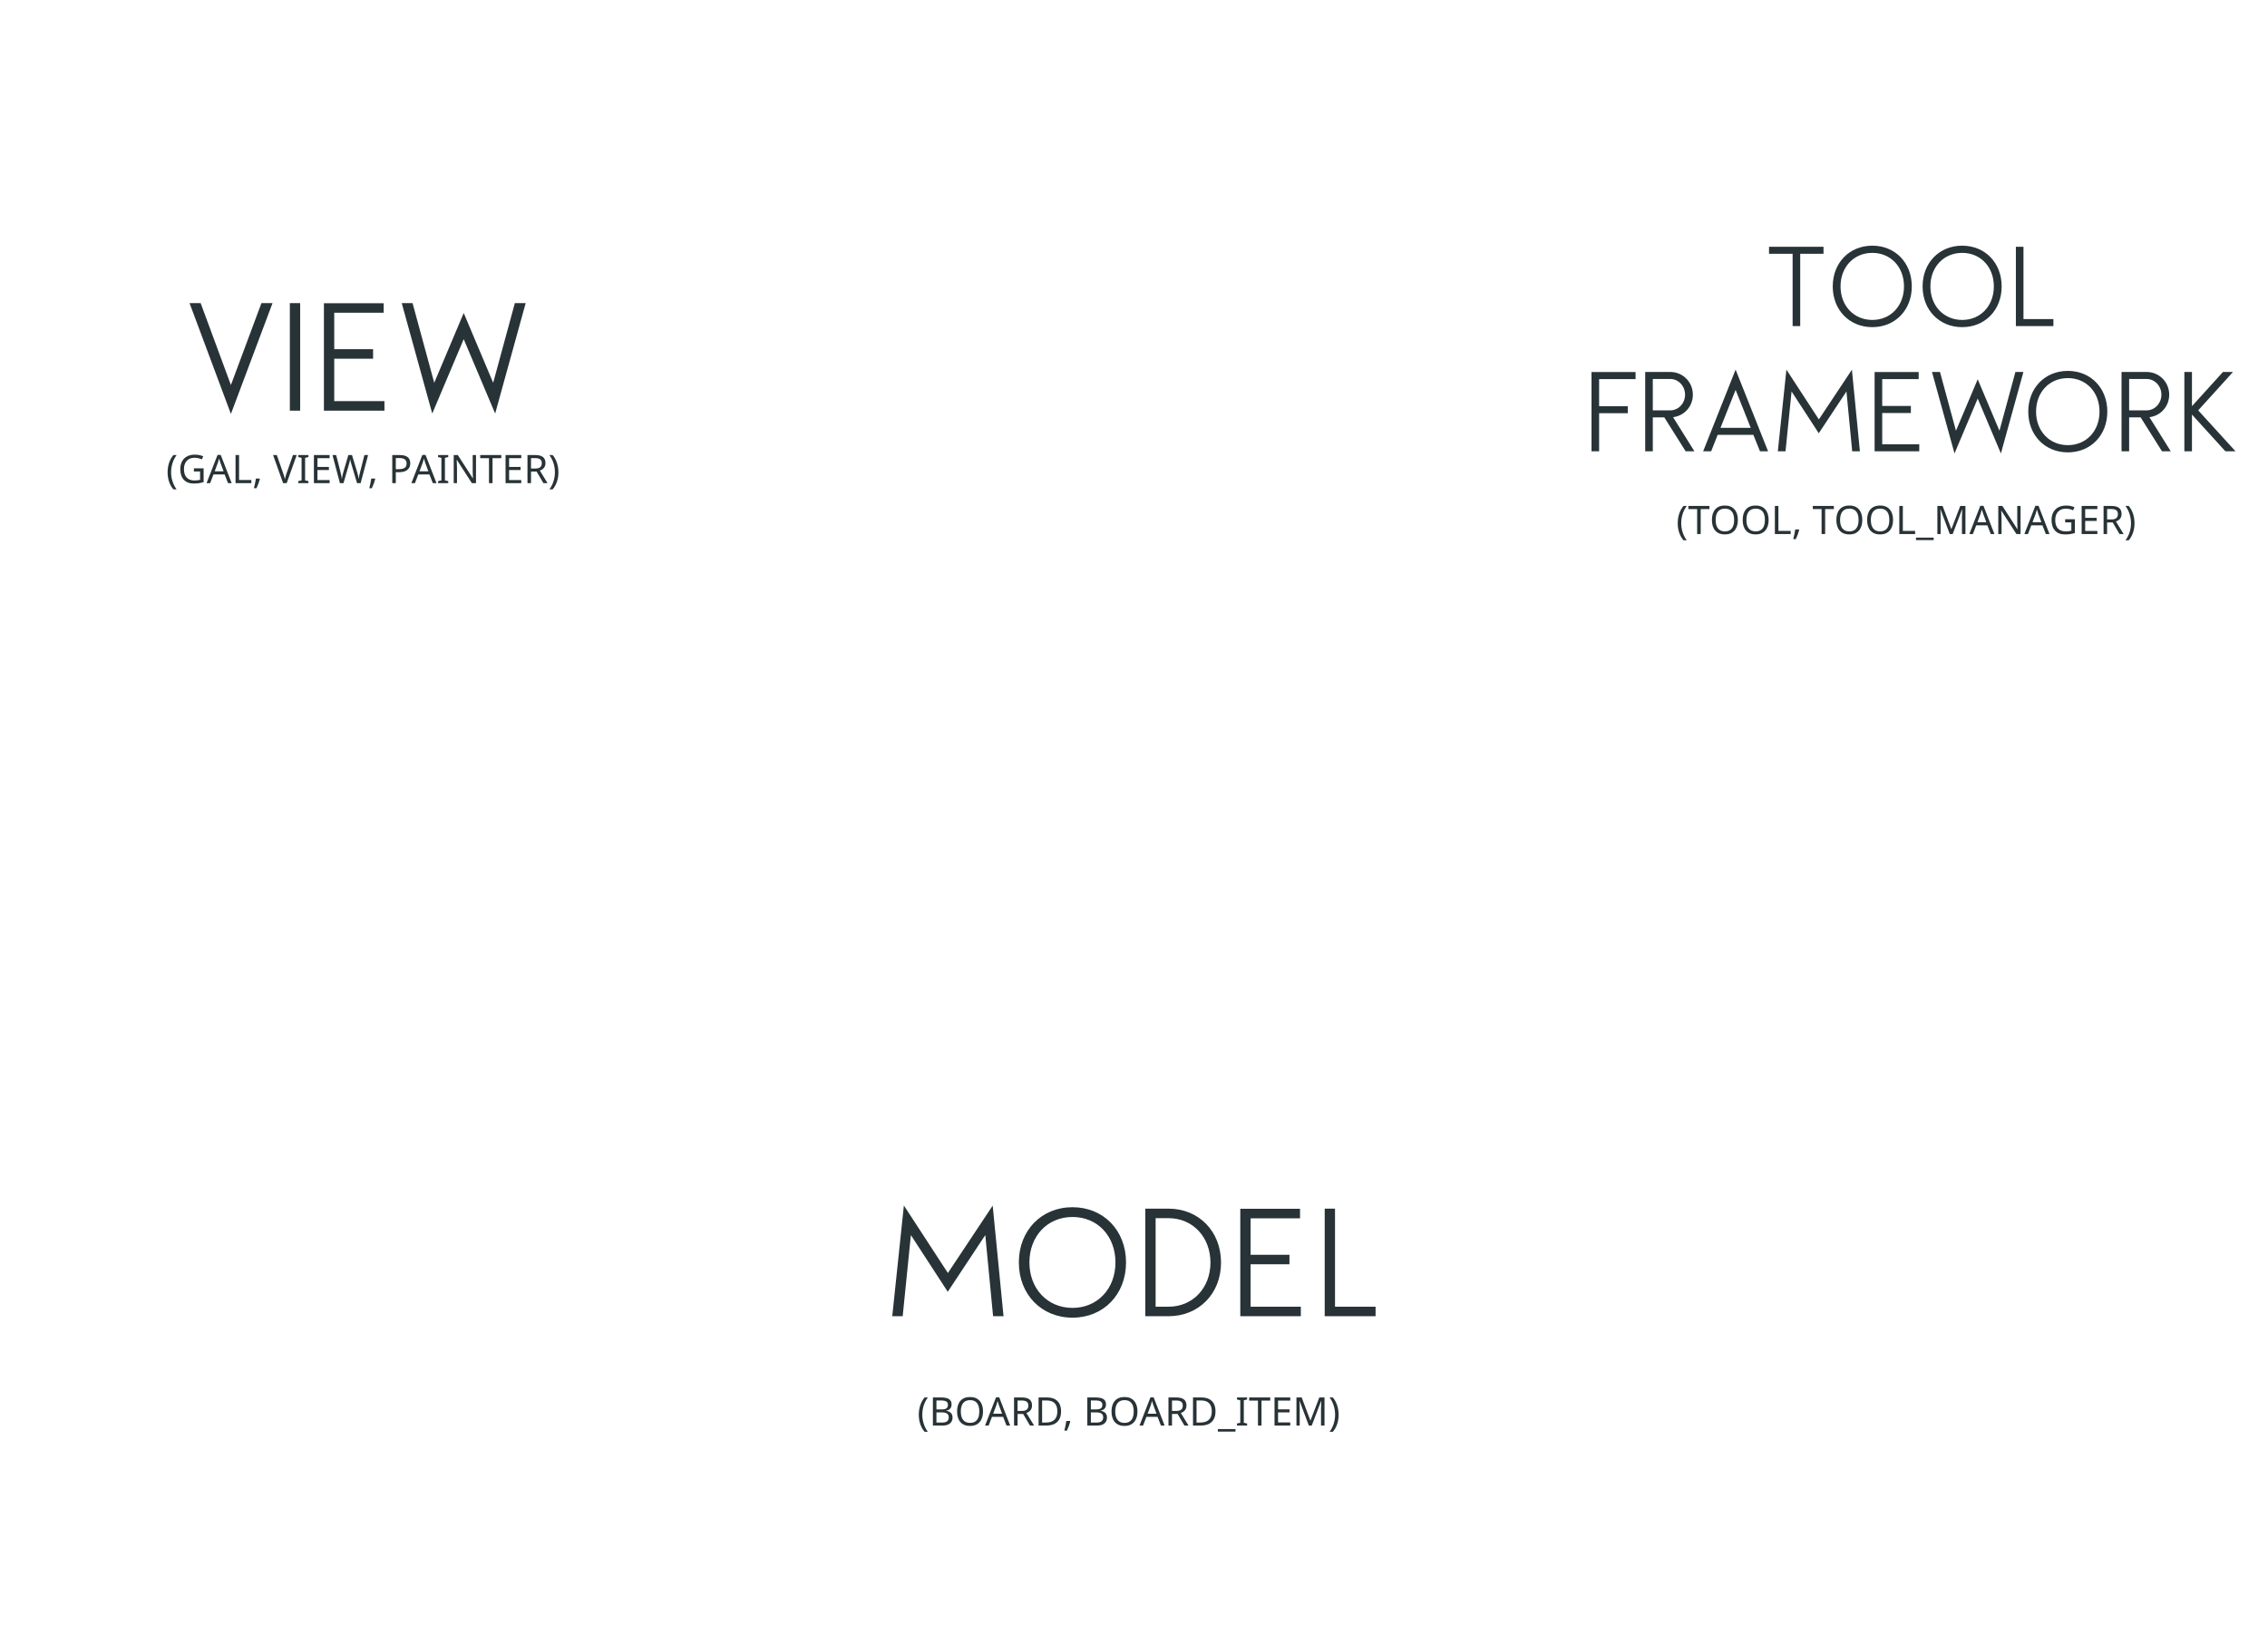
\includegraphics[width=0.8\textwidth]{gfx/tool_framework.png}
\end{frame}


\framecard{NUEVAS HERRAMIENTAS}

\begin{frame}{Nuevas herramientas}{Esqueleto}
	\begin{center}
		\begin{minipage}{0.9\textwidth}
			\inputminted{cpp}{code/cpp/tool_skeleton.cpp}
		\end{minipage}
	\end{center}
\end{frame}

\begin{frame}{Nuevas herramientas}{Constructor y destructor}
	\begin{center}
	\begin{minipage}{0.7\textwidth}
		\inputminted{cpp}{code/cpp/tool_constructor.cpp}
	\end{minipage}
	\end{center}
\end{frame}

\begin{frame}{Nuevas herramientas}{Reset}
\begin{center}
\begin{minipage}{0.7\textwidth}
	\inputminted{cpp}{code/cpp/tool_reset.cpp}
\end{minipage}
\end{center}
\end{frame}

\begin{frame}{Nuevas herramientas}{Inicialización}
\begin{center}
\begin{minipage}{0.7\textwidth}
	\inputminted{cpp}{code/cpp/tool_init.cpp}
\end{minipage}
\end{center}
\end{frame}

\begin{frame}{Nuevas herramientas}{Eventos estáticos}
\begin{center}
\begin{minipage}{0.85\textwidth}
	\inputminted{cpp}{code/cpp/tool_transitions.cpp}
\end{minipage}
\end{center}
\end{frame}

\begin{frame}{Nuevas herramientas}{Eventos interactivos}
\begin{center}
\begin{minipage}{0.8\textwidth}
	\inputminted{cpp}{code/cpp/tool_transitions_interactive.cpp}
\end{minipage}
\end{center}
\end{frame}

\framecard{C++ MOLA}

\framecard{PERO PYTHON MOLA MÁS}

\begin{frame}{Python}{Primeros pasos}
	  \begin{center}
		\begin{minipage}{0.8\textwidth}
			\inputminted[fontsize=\Large]{python}{code/python/start.py}
		\end{minipage}
	\end{center}
\end{frame}

\begin{frame}{Python}{Primeros pasos}
	\inputminted[fontsize=\large]{python}{code/python/nets.py}
\end{frame}

\begin{frame}{Python}{Primeros pasos}
\begin{center}
	\begin{minipage}{0.9\textwidth}
		\inputminted[fontsize=\large]{python}{code/python/nets2.py}
	\end{minipage}
\end{center}
\end{frame}
